\section{Most frequent integer: paired sort and scan}
\label{sec:most-frequent}

This example takes an initialized array of integers and returns its most
frequent value. An empty array returns \texttt{None}. If several values
have the same maximum frequency, the result is the value encountered first
in the original array. For example, $[8,3,3,8]$ returns $8$, even though
$3$ is numerically smaller. The input is preserved.

\paragraph{Verification status.}
Rocq checks the abstract specification, the complete functional
sort-and-scan correctness theorem, and an Iris weakest-precondition proof
of the actual CJR operation for both empty and nonempty inputs.
The proof includes allocation, input copying, paired Lomuto quicksort,
run scanning, the first-occurrence tie rule, both temporary-buffer frees,
and preservation of the input. Checked expression equalities connect the
loop lemmas to the terms supplied to the printer. The emitted Cangjie
program is compiled, tested, and benchmarked; native compilation and the
printer are outside the CJR semantic proof, as described below.

\subsection{Specification in elementary mathematics}

Let $A=(a_0,\ldots,a_{n-1})$ and define
\[
 f_A(x)=\bigl|\{i:0\leq i<n\ \land\ a_i=x\}\bigr|,
 \qquad
 t_A(x)=\min\{i:0\leq i<n\ \land\ a_i=x\}.
\]
For absent values set $t_A(x)=n$. The required answer $r$ satisfies
\[
\begin{aligned}
 r=\mathrm{None}&\quad\Longleftrightarrow\quad n=0,\\
 r=\mathrm{Some}(x)&\quad\Longrightarrow\quad
 f_A(x)>0\ \land\ (\forall y\in\mathbb Z,\ f_A(y)\leq f_A(x))\\
 &\hspace{36mm}\land\
 (\forall y\in\mathbb Z,\ f_A(y)=f_A(x)\Rightarrow t_A(x)\leq t_A(y)).
\end{aligned}
\]
Among maximum-frequency values the first-index condition determines a
unique value: different values cannot occupy the same original index.

\paragraph{English readout.}
Return no value exactly when the input is empty. Otherwise return a value
that occurs in the input, occurs at least as often as every other integer,
and whose first occurrence is no later than the first occurrence of any
other equally frequent value. Comparing only values, or returning the
first group in numeric sort order, would violate this contract.

\subsection{Gallina specification}

The executable specification uses \texttt{count\_occ} for frequency and a
recursive search for the first index; \texttt{mf\_first\_index\_or\_len}
returns the array length for an absent value. Indices and counts are
natural numbers. Values are unbounded Rocq integers.
\begin{lstlisting}
Definition most_frequent_spec (xs : list Z) (answer : option Z) : Prop :=
  match xs, answer with
  | [], None => True
  | [], Some _ => False
  | _ :: _, None => False
  | _ :: _, Some x =>
      (mf_frequency x xs > 0)%nat /\
      (forall y, mf_frequency y xs <= mf_frequency x xs)%nat /\
      (forall y, mf_frequency y xs = mf_frequency x xs ->
         mf_first_index_or_len x xs <= mf_first_index_or_len y xs)%nat
  end.
\end{lstlisting}
The independently proved \texttt{mf\_choose xs xs} computes this answer by
counting each candidate against the whole input. It is a quadratic
reference oracle, not the efficient implementation. Its theorem
\texttt{mf\_choose\_correct} proves the specification by induction over
candidate order, retaining the earlier candidate on a frequency tie.

The verified functional implementation composes paired Lomuto sort,
adjacent-value grouping, and summary selection. Written with
\texttt{option\_map} in place of the equivalent source infix notation:
\begin{lstlisting}
Definition mf_sort_scan xs : option Z :=
  option_map fst (mf_best_summary (mf_run_summaries (mf_sorted_pairs xs))).

Theorem mf_sort_scan_correct xs :
  most_frequent_spec xs (mf_sort_scan xs).
\end{lstlisting}
This theorem has no summary-validity hypothesis: the grouping and sorting
proofs discharge it. It also includes the empty case and the specified
tie rule. The CJR refinement theorem below connects the concrete operation to this functional result.

\subsection{Algorithm walkthrough and pseudocode}

Copy the input into records $(a_i,i)$, represented by two parallel arrays.
Sorting these records lexicographically places equal values together and
orders their original indices within each group. Every swap moves both
fields. For $[8,3,3,8]$, the sorted records are
$[(3,1),(3,2),(8,0),(8,3)]$. Their summaries are $(3,2,1)$ and $(8,2,0)$,
where each triple is (value, count, first index). Both counts are two; the
second summary wins because index zero precedes index one.

\begin{lstlisting}
mostFrequent(A):
  n := length(A)
  if n = 0: return None
  values := copy(A); indices := [0, ..., n-1]
  quicksortPairs(values, indices, 0, n)  // half-open interval
  bestCount := 0; bestFirst := n; start := 0
  while start < n:
    x := values[start]; end := start + 1
    first := indices[start]
    while end < n:
      if values[end] != x: break
      first := min(first, indices[end]); end := end + 1
    count := end - start
    if count > bestCount or
       (count = bestCount and first < bestFirst):
      bestValue := x; bestCount := count; bestFirst := first
    start := end
  free(values.data); free(indices.data)
  return Some(bestValue)
\end{lstlisting}
Lomuto partition uses the last record as pivot. It maintains a boundary
$i$ and visits records $j$ from \texttt{lo} through \texttt{hi-2}; records
at most the pivot are swapped into the left prefix. The pivot is then
swapped into position $i$. Recursion sorts $[\texttt{lo},i)$ and
$[i+1,\texttt{hi})$, leaving the pivot out of both recursive calls.

Under the usual random-order assumption for the distinct paired keys,
quicksort takes expected $O(n\log n)$ comparisons; its worst case is
$O(n^2)$. This implementation does not randomize pivots. Sorted,
reverse-sorted, and all-equal \emph{value} inputs can be particularly poor:
in the all-equal case the increasing original indices already put the
paired keys in sorted order. Copying and scanning take $O(n)$. The two
buffers require $O(n)$ space; recursive stack depth is $O(n)$ in the worst
case. Both raw buffers are freed before returning.

\subsection{Formal CJR implementation and emitted Cangjie}

The implementation lives in \texttt{theories/examples/most\_frequent.v}
as core-language expressions \texttt{mf\_swap\_body},
\texttt{mf\_partition\_body}, \texttt{mf\_qsort\_body}, and
\texttt{mf\_body}. A pair comparison is expressed using the available
\texttt{LeOp} and \texttt{If}; it never subtracts two input values or adds
one to an input value, so comparisons also work at the \texttt{Int64}
boundaries. The group condition uses an explicit \texttt{If} because CJR's
\texttt{AndOp} evaluates both operands. An eager conjunction containing a
raw read at \texttt{end == n} would access beyond the array.

\begin{lstlisting}
If (BinOp LeOp (Var "v") (Var "pv"))
  (If (BinOp LeOp (Var "pv") (Var "v"))
    (BinOp LeOp (Var "ix") (Var "pi"))
    (Val (LitV (LitBool true))))
  (Val (LitV (LitBool false)))
\end{lstlisting}
The following is the complete core-language definition of the pair swap,
partition, recursive sort, copy, and group scan. Calls package their
arguments in a structural value, \texttt{VarBind} introduces mutable stack
variables, and \texttt{Assign} updates those variables. The loop guards,
array reads, and final block frees are therefore explicit syntax subject
to the CJR semantics.
\lstinputlisting[firstline=179,lastline=269,basicstyle=\ttfamily\footnotesize]{theories/examples/most_frequent.v}

The printer uses these expressions directly through
\texttt{p\_most\_frequent}; \texttt{make cj} regenerates the following
standalone program. \texttt{Int64Option(false,0)} represents
\texttt{None}; its numeric field has no meaning in that case.
\lstinputlisting{generated/cj/most_frequent.cj}

The input must have a correct length and valid initialized storage at
every in-range index. The empty case reads only the length field and
allocates no temporary buffers. The tests construct an empty view over a
positive allocation instead of depending on \texttt{malloc(0)}. The full
native storage contract also requires allocation byte sizes and indices
to fit their machine types. As elsewhere in this tutorial, a Rocq proof
over unbounded integers does not by itself establish the compiler's
\texttt{Int64} arithmetic and allocation behavior.

\subsection{Correctness argument and checked components}

\paragraph{Record preservation.}
\texttt{mf\_pair\_swap\_perm} proves that swapping two records preserves
the record multiset, including self-swaps and out-of-range no-op cases in
the functional model. Induction on partition fuel lifts this to
\texttt{mf\_lomuto\_perm}. The final pivot swap preserves the same
multiset, proving \texttt{mf\_partition\_perm}. Induction on recursive
fuel composes the two recursive permutations and the partition
permutation, proving \texttt{mf\_qsort\_perm}. It follows that no original
(value,index) record is lost or duplicated by the functional sort.

\paragraph{Ordering.}
For a positive width $w$ larger than every record index, define the
\emph{proof-only} rank $\rho_w(x,i)=xw+i$. If $x<y$, then
$\rho_w(x,i)<\rho_w(y,j)$ because $0\leq i,j<w$; if $x=y$, comparing ranks
is exactly comparing indices. Conversely, a rank comparison cannot put a
larger value before a smaller value, since an index difference has
magnitude less than $w$. Lemma \texttt{mf\_rank\_order} checks this
argument with integer arithmetic. Lemmas \texttt{mf\_swap\_map},
\texttt{mf\_lomuto\_map}, \texttt{mf\_partition\_map}, and
\texttt{mf\_qsort\_slice\_map} show that mapping records to ranks commutes
with the actual functional Lomuto operations. The existing scalar
quicksort ordering theorem therefore yields \texttt{mf\_qsort\_sorted}.
For input records, \texttt{mf\_pairs\_bounded} supplies $w=n$ when $n>0$.
No rank is computed in the emitted program.

\paragraph{Frequency and provenance.}
\texttt{mf\_pairs\_values} proves that projecting original records gives
exactly the input. Mapping the sort permutation through that projection
preserves every frequency, which is
\texttt{mf\_sorted\_pairs\_frequency}. The lookup lemma and permutation
also prove \texttt{mf\_sorted\_pairs\_origin}: every sorted record's
index points to its value in the original input. This is stronger than
preserving a multiset of values alone.

\paragraph{Grouping obligation.}
In a lexicographically sorted record sequence, all records with value $x$
form one contiguous run. A different value between two $x$ records would
have to be both at least $x$ and at most $x$, contradicting its difference.
Scanning from the run's first record until the first different value
therefore visits exactly all $x$ records. Its length is $f_A(x)$ and the
minimum original index is $t_A(x)$. To mechanize the imperative scan, the
inner invariant must state that $[\texttt{start},\texttt{end})$ is exactly
the portion of this run already visited, and that \texttt{first} is the
minimum index there. It must also retain ownership of both buffers and
establish each read is in bounds. The functional grouping is now checked: \texttt{mf\_run\_summaries\_sound} proves that each summary has its global
frequency, a witnessed minimum original index, and positive count, that
summary keys do not repeat, and that all record values are represented.
The functional scan builds the same adjacent-value groups by structural
recursion from the tail, extending the first summary when its value agrees
with the current record. Its induction uses sortedness to exclude an
earlier value from every later, different-value group. The forward-loop invariant and its refinement of this grouping are proved
by the concrete scan lemmas described below.

\paragraph{Selection.}
A summary $s$ has value, count, and first-index fields. Its score is better
than another summary when its count is larger, or its count is equal and
its first index is no larger. The checked lemmas establish a total,
transitive score order. \texttt{mf\_best\_summary\_sound} proves by
induction that the selected summary belongs to the list and dominates
every other summary. The theorem \texttt{mf\_summary\_selection\_correct}
then establishes \texttt{most\_frequent\_spec}, provided all summaries
have their true positive frequencies and first indices, and every input
value has a summary. Absent values have frequency zero, so the domination
condition extends to all integers. The checked theorem \texttt{mf\_run\_summaries\_complete} now establishes
that precondition for the actual functional groups of the paired sort.
Permutation transfers the minimum-index witnesses back to the original
input; \texttt{mf\_first\_index\_attained} and
\texttt{mf\_first\_index\_minimum} show that this minimum is exactly the
specification's first-occurrence index. Composing these results gives
\texttt{mf\_sort\_scan\_correct}, a correctness theorem for the complete
functional algorithm rather than only the independent quadratic oracle.

\paragraph{Concrete paired-array Iris proof.}
The predicate \texttt{mf\_pair\_arrays ps oa ob} owns two initialized arrays:
one contains the value projection of the record list, and the other
contains the original-index projection, embedded from naturals into
integers. \texttt{mf\_swap\_arrays\_wp} checks all four reads and all four
writes of the actual swap body. On a self-swap the two initial lookup
facts imply the read values agree, which justifies the second write after
the first update. Mapping the functional record swap through both
projections gives \texttt{mf\_swap\_pairs\_wp}.

\texttt{mf\_lex\_compare\_wp} proves the concrete nested comparisons return
exactly \texttt{mf\_pair\_leb}. Each partition iteration reads the current
record, applies this comparison, optionally swaps it into the stored
prefix and increments $i$, then increments $j$.
\texttt{mf\_partition\_step\_wp} accounts for both arrays and both mutable
stack cells throughout that step. Induction on the remaining scan length,
$(\texttt{hi}-1)-j$, yields \texttt{mf\_partition\_scan\_wp}: its result is
exactly the functional \texttt{mf\_lomuto} result and its final $j$ is
\texttt{hi-1}. The induction maintains $i\leq j\leq\texttt{hi-1}$ and
\texttt{hi-1} below the array length, so both record reads and swaps are
in bounds. Equality lemmas extract the loop directly from
\texttt{mf\_partition\_body} and check that it is the expression proved by
these step and scan theorems.

\texttt{mf\_partition\_wp} opens the two local stack variables, reads the
last record as pivot, applies the scan theorem, performs the final pivot
swap, and returns the functional partition index. It returns both array
representations and supplies the stack cells for their lexical scope
cleanup. The bound $\texttt{lo}\leq p<\texttt{hi}$ makes both recursive
subintervals strictly shorter. Induction on a fuel at least
$\texttt{hi}-\texttt{lo}$ then proves \texttt{mf\_qsort\_slice\_wp} for the
actual recursive CJR function. Its postcondition is the exact functional
\texttt{mf\_qsort\_slice} array contents, not merely an assertion that some
sorted list exists. At full length, \texttt{mf\_qsort\_wp} therefore connects
the emitted paired quicksort to the previously proved sorted-permutation
model. No abstract comparator or swap correctness is assumed here.

\paragraph{Complete-buffer cleanup.}
The new \texttt{mf\_wp\_free\_block} rule owns a block token for the exact
buffer length and all of its raw cells. Its proof deletes the cells in
reverse index order from the Iris ghost map, deletes the block token,
and uses \texttt{mf\_wf\_free\_block} to preserve the state invariant.
Disjoint live blocks retain their cells: the deleted interval cannot
intersect any of their intervals. \texttt{mf\_release\_array\_wp} applies
this rule to the actual \texttt{Free(FieldLoad(array,1))} expression.
\texttt{mf\_cleanup\_wp} composes the two final frees and result
construction while framing ownership of the unchanged input array.
The cleanup preserves the already selected scalar value; it reads no
buffer cell after freeing a buffer.

\paragraph{Copying and initialization.}
For input $A$ of length $n$, after $j$ copy iterations in the CJR
allocation model the value buffer is
\[
 \mathrm{take}(j,A)\mathbin{+\!+}\mathrm{replicate}(n-j,0),
\]
and the index buffer is $[0,\ldots,j-1]$ followed by $n-j$ zero cells.
The zero suffix describes the modeled allocation. The emitted native
routine writes every temporary cell before reading it, so this operation
does not rely on \texttt{malloc} returning zeroed memory.
The initialized prefix grows by one cell on each iteration. The loop
condition supplies $j<n$, justifying the source read and both destination
writes. Ownership of the input is retained throughout. At $j=n$, the
buffers are exactly the two projections of \texttt{mf\_pairs A 0}.
\texttt{mf\_copy\_step\_wp} proves the actual nested read/write step;
\texttt{mf\_copy\_loop\_wp} proves the loop by induction on $n-j$.
\texttt{mf\_copy\_loop\_is\_code} is an expression equality obtained from
\texttt{mf\_body}, so a separate copy program cannot satisfy this proof
in place of the emitted one.

\paragraph{Concrete run and winner scan.}
The pure helper \texttt{mf\_scan\_run value first suffix} returns the
number of additional equal-value records and the minimum original index
including the already visited records. It stops on an empty suffix or a
different value. \texttt{mf\_group\_inner\_wp} proves the actual guarded
inner loop computes exactly this pair: if the loop starts at position
$j$ with minimum $t$, it finishes at $j+\mathrm{extra}$ with the computed
minimum. Its induction follows the unread suffix. An exhausted suffix
implies $j=n$; the explicit conditional returns false without loading a
cell. A nonempty suffix implies $j<n$, so the equality test is safe.
On a matching record, the index read is safe, the conditional minimum
update preserves its stack cell, and advancing the cursor decreases the
unread suffix. A different value leaves the cursor and minimum unchanged.
The theorem retains both arrays and both mutable stack cells in every case.

\texttt{mf\_group\_summary\_decomposition} connects this forward scan
to \texttt{mf\_run\_summaries}: for a first record $p$ and suffix $P$,
scanning the additional equal records produces the first summary
$(p.\mathrm{value},1+\mathrm{extra},\mathrm{minimum})$, and the remaining
summaries are exactly those of the suffix after dropping those records.
The proof combines adjacent summaries; count addition and minimum are
associative. Thus the forward implementation and the tail-recursive
functional grouping agree, without assuming that agreement as a precondition.

\texttt{mf\_strict\_better} uses a larger count, or an equal count and a
strictly smaller first index, exactly as the native operation does.
\texttt{mf\_fold\_best\_sound} proves that the accumulated winner is one
of the seed and processed summaries and dominates all of them in the
score order. The seed has count zero. Every real summary has positive
count, so a nonempty completed scan cannot select the seed.
\texttt{mf\_forward\_scan\_correct} combines this fact, completeness of
all run summaries, and the score order to prove the specification.

The concrete update lemmas prove the nested count/tie comparison and all
three assignments to the best-value, best-count, and best-first stack cells.
\texttt{mf\_group\_step\_wp} composes the first-record reads, creation of
local end/minimum cells, inner loop, summary selection, and cursor update.
It also returns the local stack ownership required for scope cleanup.
\texttt{mf\_group\_outer\_wp} proves the full outer loop by induction
on a fuel at least the unread suffix length. Each iteration consumes at
least its first record; its next cursor is in bounds and its remaining
suffix is shorter. Its final best cells contain the exact
\texttt{mf\_forward\_scan} result. Checked expression equalities link
both loops to \texttt{mf\_body}.

\paragraph{Complete Iris contract.}
The input predicate handles the empty header separately because the
CJR raw-allocation model requires positive block lengths:
\begin{lstlisting}
Definition mf_input `{!cjrGS Σ} (xs : list Z) oi : iProp Σ :=
  match xs with
  | [] => ObjId oi ↦ₒ[0] LitV (LitInt 0)
  | _ :: _ => is_array xs (LitV (LitObj oi))
  end.
\end{lstlisting}
Here $\mapsto_o[0]$ denotes ownership of object field zero. The empty case requires only the zero length field because the
operation reads no element or pointer and allocates nothing.
The positive case owns the initialized input array, including its exact
length, data pointer, raw-block token, and element cells.
\texttt{mf\_option\_value} encodes \texttt{None} as the false/zero result
structure and \texttt{Some x} as the true/$x$ structure.
The checked complete theorem is
\[
 \mathrm{mfInput}(A,a)\ \vdash\
 \mathrm{WP}\ \mathrm{mostFrequent}(a)\
 \{v.\ \lceil v=\mathrm{encode}(\mathrm{mfSortScan}(A))\rceil
       *\mathrm{mfInput}(A,a)\}.
\]
\par\noindent
\begin{minipage}{\textwidth}
\begin{lstlisting}
Theorem mf_wp `{!cjrGS Σ} `{!invGS_gen HasLc Σ} xs oi :
  mf_input xs oi -∗
  WP App (Rec None (Some "input") mf_body) (Val (LitV (LitObj oi)))
    {{ v, ⌜v = mf_option_value (mf_sort_scan xs)⌝ ∗ mf_input xs oi }}.
\end{lstlisting}
\end{minipage}\par
The connective $-\!* $ is separating implication: it consumes the
input ownership to establish the weakest-precondition assertion. The
postcondition combines a pure result equality with ownership of the same
input using separating conjunction.
\texttt{mf\_nonempty\_wp} proves allocation of two positive-length
buffers, applies the copy and quicksort theorems, initializes the winner
and cursor cells, then applies the outer scan theorem. The actual final
\texttt{Free} expressions consume both temporary raw buffers. The result
is read from the best-value stack cell after cleanup. The input ownership
is framed throughout and returned unchanged. The proof supplies all local
stack cells for lexical scope cleanup.
\texttt{most\_frequent\_spec\_unique} shows that two answers satisfying
the specification are equal: their maximum frequencies agree, their first
indices agree, and the input cell at that index determines their value.
It identifies the forward scan's answer with \texttt{mf\_sort\_scan}.
\texttt{mf\_wp} combines this nonempty proof with \texttt{mf\_empty\_wp};
\texttt{mf\_spec\_wp} adds the specification to its postcondition.
No copying, grouping, comparator, or sorting hypothesis is assumed for
this contract. The representative project assumption audit checks
73 theorems, including the complete operation and its kernels.

\subsection{Testing and comparative benchmarks}

Eleven Cangjie unit-test methods pass against the emitted source: empty,
singleton, all-equal, all-distinct, interleaved two-way and three-way ties,
negative and boundary integers, sorted and reversed inputs, exhaustive
small arrays, and paired-sort preservation. The exhaustive test checks all
3,280 arrays of lengths zero through seven over $\{-1,0,1\}$ against an
independent quadratic reference. Every result test also checks that the
input is unchanged. The pair test checks lexicographic order, distinct
original indices, and each value's correspondence to its original index.
Tests check native behavior in addition to the CJR refinement proof;
they do not prove the printer or native compiler correct.

The baselines are explicitly written equivalent operations using the
SDK's \texttt{std.sort.sort} and \texttt{std.collection.HashMap}. They
are not built-in most-frequent functions. The sort baseline sorts an array
of original indices with a value/index comparator and scans equal-value
runs. The HashMap baseline counts and maintains the maximum count in one
pass, then visits the original input until it finds a value with that
count, preserving first-occurrence semantics. All return the same option
encoding, preserve the input, and check the empty case.

The compiler is Cangjie 1.0.5 cjnative at \texttt{-O2}, targeting
\texttt{aarch64-apple-darwin}, on an Apple M4 Mac mini with 16 GB RAM and
macOS 26.6.2. Three independent sequential processes each record seven
samples per implementation at each workload/size point: 693 measurements
in total. Each operation receives identical preconstructed values. Timing
includes its allocations, copying or map construction, sorting/counting,
scan, result construction, and the CJR buffer frees. Input setup, warmups,
checksums, and printing are outside the timer. Each implementation receives
two warmup calls. Batch repetitions are $262144/n$ for all implementations;
trial order rotates through the three implementations. There is no core
pinning, forced garbage collection, or subtraction of loop overhead.

The deterministic distributions are
$a_i=((37i)\bmod101)-50$ (dense),
$a_i=((48271i)\bmod n)-n/2$ (distinct permuted values), and
$a_i=((17i)\bmod7)-3$ (seven values), at $n=256,4096,16384$.
Sorted and reverse-sorted distinct inputs are measured only at $n=256$
to bound the cost of the deliberately reused quadratic worst case.
These workloads are not random samples from all input distributions.
Raw results, source hashes, compiler metadata, and reproducible runners
are in \texttt{benchmark/results/most\_frequent/} and
\texttt{benchmark/most\_frequent\_run.py}.

\begin{figure}[H]
\centering
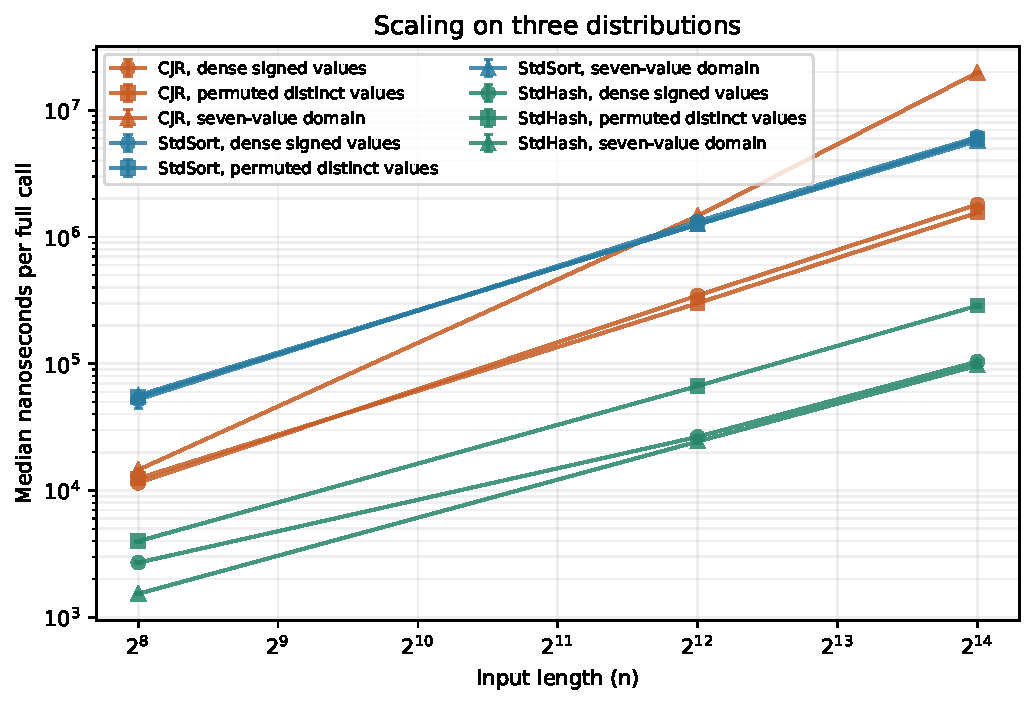
\includegraphics[width=\textwidth]{paper/figures/most-frequent-scaling.pdf}
\caption{Complete-operation timings: median elapsed time per call;
error bars show the interquartile range across 21 samples.}
\label{fig:most-frequent-benchmark}
\end{figure}
\begin{figure}[H]
\centering
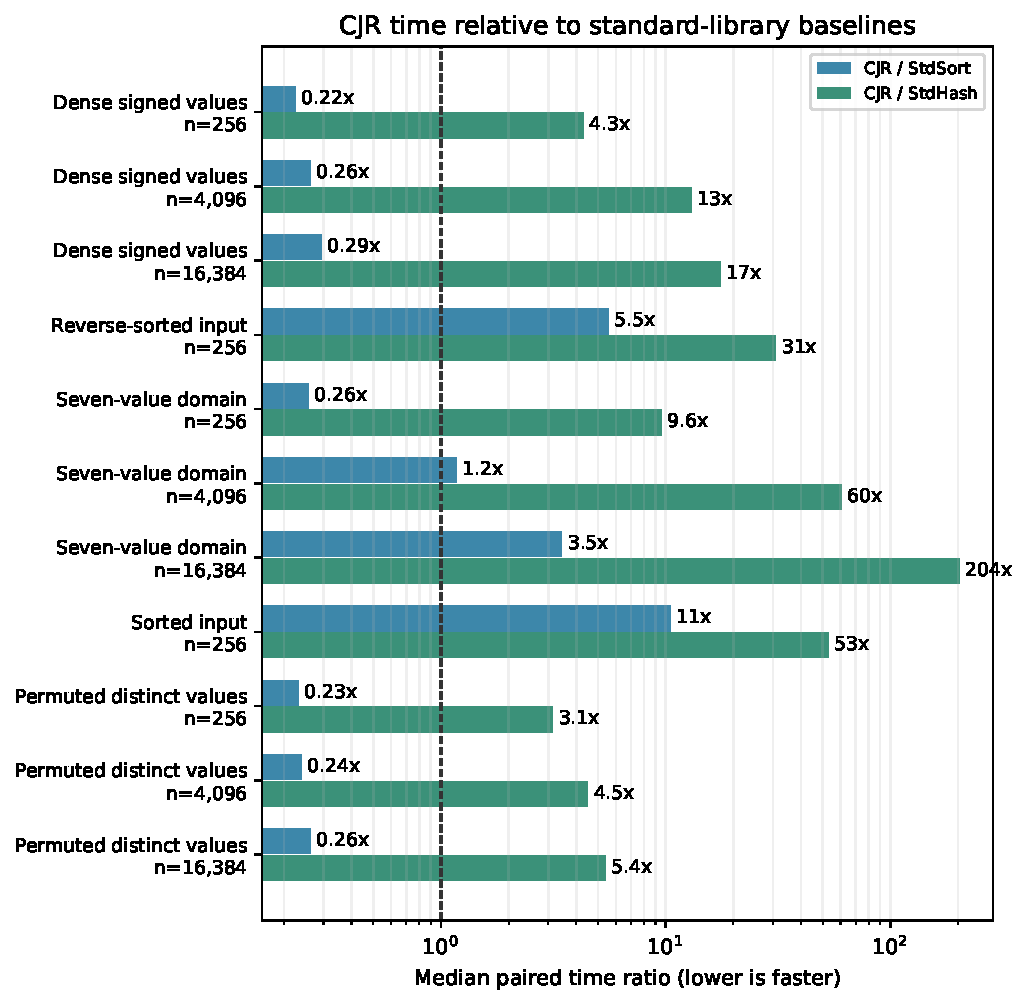
\includegraphics[width=\textwidth]{paper/figures/most-frequent-ratios.pdf}
\caption{Median paired CJR/baseline ratios. Values above one mean CJR is slower.}
\end{figure}
\begin{table}[H]
\centering\small
\begin{tabular}{lrrrr}
\hline
Distribution & $n$ & CJR ($\mu$s) & std.sort ($\mu$s) & HashMap ($\mu$s) \\
\hline
Dense signed values & 256 & 11.47 & 52.21 & 2.69 \\
Dense signed values & 4,096 & 345.78 & 1,325.61 & 26.50 \\
Dense signed values & 16,384 & 1,802.94 & 6,134.94 & 103.88 \\
Reverse-sorted input & 256 & 124.43 & 22.44 & 4.01 \\
Seven-value domain & 256 & 14.54 & 56.32 & 1.53 \\
Seven-value domain & 4,096 & 1,468.05 & 1,250.11 & 24.33 \\
Seven-value domain & 16,384 & 19,752.75 & 5,718.88 & 96.69 \\
Sorted input & 256 & 207.17 & 19.75 & 3.91 \\
Permuted distinct values & 256 & 12.46 & 54.51 & 3.98 \\
Permuted distinct values & 4,096 & 300.00 & 1,256.50 & 66.67 \\
Permuted distinct values & 16,384 & 1,553.56 & 5,954.69 & 287.00 \\
\hline
\end{tabular}
\caption{Median time per complete operation; 21 samples per entry.}
\end{table}


These measurements compare complete implementations with different
representations and runtime costs. CJR uses unchecked raw accesses; the
sort baseline uses standard arrays and a comparator that reads the input
through their API. CJR allocates two buffers whereas that baseline
allocates one index array. Consequently a speed difference does not
isolate the sorting algorithm. The seven-value and already ordered cases
expose the pivot strategy's weakness. The HashMap alternative avoids
sorting and can be substantially faster, but relies on hashing behavior
and a different verification effort. No timing establishes correctness,
a general performance ranking, or worst-case bounds for the SDK's map.
